


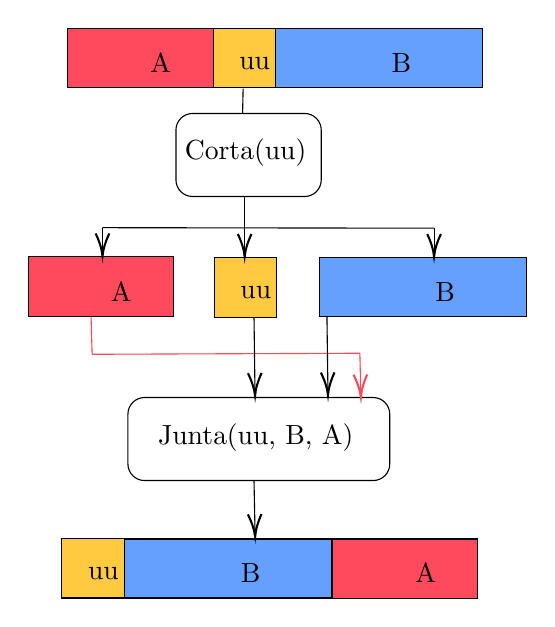
\begin{tikzpicture}[x=0.75pt,y=0.75pt,yscale=-1,xscale=1]
%uncomment if require: \path (0,300); %set diagram left start at 0, and has height of 300

%Shape: Rectangle [id:dp23098094173558026] 
\draw  [fill={rgb, 255:red, 255; green, 73; blue, 92 }  ,fill opacity=1 ] (149.02,2.79) -- (219.02,2.79) -- (219.02,31.54) -- (149.02,31.54) -- cycle ;
%Shape: Rectangle [id:dp6390512458709207] 
\draw  [fill={rgb, 255:red, 102; green, 160; blue, 255 }  ,fill opacity=1 ] (249.19,3.12) -- (348.97,3.12) -- (348.97,31.54) -- (249.19,31.54) -- cycle ;
%Shape: Rectangle [id:dp6196376467227851] 
\draw  [fill={rgb, 255:red, 255; green, 202; blue, 64 }  ,fill opacity=1 ] (219.02,2.87) -- (249.19,2.87) -- (249.19,31.54) -- (219.02,31.54) -- cycle ;
%Shape: Rectangle [id:dp8865869608598624] 
\draw  [fill={rgb, 255:red, 255; green, 73; blue, 92 }  ,fill opacity=1 ] (129.97,112.81) -- (199.97,112.81) -- (199.97,141.56) -- (129.97,141.56) -- cycle ;
%Shape: Rectangle [id:dp7413739983750511] 
\draw  [fill={rgb, 255:red, 102; green, 160; blue, 255 }  ,fill opacity=1 ] (270.36,113.14) -- (370.14,113.14) -- (370.14,141.56) -- (270.36,141.56) -- cycle ;
%Shape: Rectangle [id:dp3646083407953362] 
\draw  [fill={rgb, 255:red, 255; green, 202; blue, 64 }  ,fill opacity=1 ] (219.53,113.33) -- (249.69,113.33) -- (249.69,142) -- (219.53,142) -- cycle ;
%Shape: Rectangle [id:dp8914572744141535] 
\draw  [fill={rgb, 255:red, 102; green, 160; blue, 255 }  ,fill opacity=1 ] (176.56,248.9) -- (276.34,248.9) -- (276.34,277.31) -- (176.56,277.31) -- cycle ;
%Shape: Rectangle [id:dp3986048597954386] 
\draw  [fill={rgb, 255:red, 255; green, 202; blue, 64 }  ,fill opacity=1 ] (146.17,248.65) -- (176.34,248.65) -- (176.34,277.31) -- (146.17,277.31) -- cycle ;
%Shape: Rectangle [id:dp1189549985165792] 
\draw  [fill={rgb, 255:red, 255; green, 73; blue, 92 }  ,fill opacity=1 ] (276.34,248.9) -- (346.34,248.9) -- (346.34,277.65) -- (276.34,277.65) -- cycle ;
%Rounded Rect [id:dp24586206145017386] 
\draw   (201.14,51.86) .. controls (201.14,47.44) and (204.72,43.86) .. (209.14,43.86) -- (263.14,43.86) .. controls (267.56,43.86) and (271.14,47.44) .. (271.14,51.86) -- (271.14,75.86) .. controls (271.14,80.28) and (267.56,83.86) .. (263.14,83.86) -- (209.14,83.86) .. controls (204.72,83.86) and (201.14,80.28) .. (201.14,75.86) -- cycle ;
%Rounded Rect [id:dp044983850626901245] 
\draw   (178,188.71) .. controls (178,184.3) and (181.58,180.71) .. (186,180.71) -- (296.14,180.71) .. controls (300.56,180.71) and (304.14,184.3) .. (304.14,188.71) -- (304.14,212.71) .. controls (304.14,217.13) and (300.56,220.71) .. (296.14,220.71) -- (186,220.71) .. controls (181.58,220.71) and (178,217.13) .. (178,212.71) -- cycle ;
%Straight Lines [id:da9018859190325679] 
\draw    (233.5,31.88) -- (233.25,43.88) ;
%Straight Lines [id:da4896523108518228] 
\draw    (165.75,98.88) -- (165.75,110.63) ;
\draw [shift={(165.75,112.63)}, rotate = 270] [color={rgb, 255:red, 0; green, 0; blue, 0 }  ][line width=0.75]    (10.93,-3.29) .. controls (6.95,-1.4) and (3.31,-0.3) .. (0,0) .. controls (3.31,0.3) and (6.95,1.4) .. (10.93,3.29)   ;
%Straight Lines [id:da2681283034938149] 
\draw    (234.25,83.88) -- (234.25,110.88) ;
\draw [shift={(234.25,112.88)}, rotate = 270] [color={rgb, 255:red, 0; green, 0; blue, 0 }  ][line width=0.75]    (10.93,-3.29) .. controls (6.95,-1.4) and (3.31,-0.3) .. (0,0) .. controls (3.31,0.3) and (6.95,1.4) .. (10.93,3.29)   ;
%Straight Lines [id:da28728594489092973] 
\draw    (325.5,99.13) -- (325.5,110.88) ;
\draw [shift={(325.5,112.88)}, rotate = 270] [color={rgb, 255:red, 0; green, 0; blue, 0 }  ][line width=0.75]    (10.93,-3.29) .. controls (6.95,-1.4) and (3.31,-0.3) .. (0,0) .. controls (3.31,0.3) and (6.95,1.4) .. (10.93,3.29)   ;
%Straight Lines [id:da9378763315903065] 
\draw    (165.75,98.88) -- (325.5,99.13) ;
%Straight Lines [id:da5499764460079808] 
\draw [color={rgb, 255:red, 255; green, 73; blue, 92 }  ,draw opacity=1 ][fill={rgb, 255:red, 255; green, 73; blue, 92 }  ,fill opacity=1 ]   (289.75,159.38) -- (290.2,178.63) ;
\draw [shift={(290.25,180.63)}, rotate = 268.65] [color={rgb, 255:red, 255; green, 73; blue, 92 }  ,draw opacity=1 ][line width=0.75]    (10.93,-3.29) .. controls (6.95,-1.4) and (3.31,-0.3) .. (0,0) .. controls (3.31,0.3) and (6.95,1.4) .. (10.93,3.29)   ;
%Straight Lines [id:da47708478900224005] 
\draw [color={rgb, 255:red, 255; green, 73; blue, 92 }  ,draw opacity=1 ][fill={rgb, 255:red, 255; green, 73; blue, 92 }  ,fill opacity=1 ]   (160.25,141.88) -- (160.75,159.88) ;
%Straight Lines [id:da21636913810049396] 
\draw [color={rgb, 255:red, 255; green, 73; blue, 92 }  ,draw opacity=1 ][fill={rgb, 255:red, 255; green, 73; blue, 92 }  ,fill opacity=1 ]   (160.75,159.88) -- (289.75,159.38) ;
%Straight Lines [id:da9036102966345168] 
\draw [color={rgb, 255:red, 0; green, 0; blue, 0 }  ,draw opacity=1 ][fill={rgb, 255:red, 255; green, 73; blue, 92 }  ,fill opacity=1 ]   (238.75,142.13) -- (239.22,177.88) ;
\draw [shift={(239.25,179.88)}, rotate = 269.24] [color={rgb, 255:red, 0; green, 0; blue, 0 }  ,draw opacity=1 ][line width=0.75]    (10.93,-3.29) .. controls (6.95,-1.4) and (3.31,-0.3) .. (0,0) .. controls (3.31,0.3) and (6.95,1.4) .. (10.93,3.29)   ;
%Straight Lines [id:da5266915850020596] 
\draw [color={rgb, 255:red, 0; green, 0; blue, 0 }  ,draw opacity=1 ][fill={rgb, 255:red, 255; green, 73; blue, 92 }  ,fill opacity=1 ]   (273.89,141.84) -- (274.37,177.59) ;
\draw [shift={(274.39,179.59)}, rotate = 269.24] [color={rgb, 255:red, 0; green, 0; blue, 0 }  ,draw opacity=1 ][line width=0.75]    (10.93,-3.29) .. controls (6.95,-1.4) and (3.31,-0.3) .. (0,0) .. controls (3.31,0.3) and (6.95,1.4) .. (10.93,3.29)   ;
%Straight Lines [id:da9952573585300807] 
\draw [color={rgb, 255:red, 0; green, 0; blue, 0 }  ,draw opacity=1 ][fill={rgb, 255:red, 255; green, 73; blue, 92 }  ,fill opacity=1 ]   (238.75,220.98) -- (239.25,245.86) ;
\draw [shift={(239.29,247.86)}, rotate = 268.86] [color={rgb, 255:red, 0; green, 0; blue, 0 }  ,draw opacity=1 ][line width=0.75]    (10.93,-3.29) .. controls (6.95,-1.4) and (3.31,-0.3) .. (0,0) .. controls (3.31,0.3) and (6.95,1.4) .. (10.93,3.29)   ;

% Text Node
\draw (187.52,13.84) node [anchor=north west][inner sep=0.75pt]   [align=left] {A};
% Text Node
\draw (303.75,13.84) node [anchor=north west][inner sep=0.75pt]   [align=left] {B};
% Text Node
\draw (230.41,15.62) node [anchor=north west][inner sep=0.75pt]   [align=left] {uu};
% Text Node
\draw (168.47,123.86) node [anchor=north west][inner sep=0.75pt]   [align=left] {A};
% Text Node
\draw (324.92,123.86) node [anchor=north west][inner sep=0.75pt]   [align=left] {B};
% Text Node
\draw (230.92,126.08) node [anchor=north west][inner sep=0.75pt]   [align=left] {uu};
% Text Node
\draw (231.12,259.62) node [anchor=north west][inner sep=0.75pt]   [align=left] {B};
% Text Node
\draw (157.56,261.4) node [anchor=north west][inner sep=0.75pt]   [align=left] {uu};
% Text Node
\draw (315.23,259.29) node [anchor=north west][inner sep=0.75pt]   [align=left] {A};
% Text Node
\draw (204.14,54.86) node [anchor=north west][inner sep=0.75pt]   [align=left] {Corta(uu)};
% Text Node
\draw (191.29,191.89) node [anchor=north west][inner sep=0.75pt]   [align=left] {Junta(uu, B, A)};


\end{tikzpicture}

